\chapter{Modeling and Controlling ATSs - The MPC for ATS and the RCS}\label{ch:mpc}
Motivated by the insights obtained in the previous chapter, which suggested that making decisions in the present have a great impact on the future, a novel model for an ATSs is proposed which, coupled with an ad-hoc designed MPC, aims at optimizing long-term outcomes by dynamically adjusting strategies in response to evolving circumstances. Furthermore, in order to improve the real-time performance of the controller, graph transformation systems are used to derive a more abstract version of the road network, named Reduced Connectivity Schema (RCS), to reduce the complexity of the model. The chapter is organized as follows:
 In \secref{sec:linear_discrete_time_model}, a novel model for the system is developed. Subsequently, \secref{sec:prob_formulat_mpc} defines the MPC problem and includes a thorough discussion on the terminal set and cost function, which are essential to prove stability. In order to achieve this goal, the feasibility of the terminal and of the states set is demonstrated. \secref{sec:gts_mpc} introduces the set of GTS rules and their condition aiming at the creation of a dynamic, adaptive and abstract representation of the road network. Finally, in \secref{sec:use_case_mpc}, a simulation is proposed to evaluate the overall performance of the system.
\section{Linear Discrete-Time Model of an ATS}\label{sec:linear_discrete_time_model}
%The model derived in this section is partially inspired from \cite{zhang2016}. \\
Consider a transportation network be composed of $|\mathcal{V}|$ stations connected by a set of $|\mathcal{N}|$ roads and $|\mathcal{A}|$ multi-occupancy, goods-carrying vehicles. Within this context, customers are assumed to requests rides only from the abovementioned stations.\\ %Similarly, goods can be carried out only from one station to another. With this assumption, stations and customers can be considered synonyms within this section. \\
Similarly to the model described in \chapref{sec:vc_model}, other than carrying goods or people, vehicle are expected to \textit{(i)} serve clients from one station to another and \textit{(ii)} reach locations in $\mathcal{V}$ in order to avoid system imbalance. For the rest of the section, a generic road $\langle i,j\rangle \in \mathcal{N}$ belonging to the network will be considered.\\
Let $d_{ij} \in \mathcal{R}_{\ge0}$ be the total lenght of a road $\langle i,j\rangle$. Let $v^a_{ij}(t) \in \{0,1\}$ indicate whether a transporting vehicle $a \in \mathcal{A}$ is moving from station $i$ to station $j$ ($v^a_{ij}(t) = 1$) and, likewise, $w^{a}_{ij}\in \{0,1\} $ whether an empty vehicle is moving from $i$ to $j$ ($w^{a}_{ij}(t)= 1$). Let $V_{ij}(t) \in \{ x \in \mathbb{N}_0 : x \leq |\mathcal{A}|\}$ being the total number of vehicles currently circulating on the street $\langle i,j\rangle$, this can be clearly expressed as in \equaref{eq:vehicles_on_street}. \\

\begin{equation}
	V_{ij}(t) = \sum_{a \in \mathcal{A}} v^{a}_{ij}(t) +w^{a}_{ij}(t)
	\label{eq:vehicles_on_street}
\end{equation}

When a vehicle is in transit, it is essential to monitor the anticipated duration until it reaches its destination. In order to do so, let's assume the road $\langle i,j\rangle$ to have a speed limit $l_{i,j}$. Accordingly, since the system is dealing with fully autonomous vehicles, in a typical driving scenario, one can safely assume this to be the cruising speed as well. In other words, one can assume the vehicles to be driving with a speed $l_{i,j}$ over $\langle i,j\rangle$ in normal road conditions. Motivated by safety concerns, the cruising speed cannot be consistently maintained at $l_{i,j}$ due to various factors. These factors may include road conditions, weather conditions, traffic density, or any unforeseen circumstances. Therefore, the actual cruising speed during the journey over road $\langle i,j\rangle$ may vary based on these dynamic elements, ensuring that the autonomous vehicles can adapt to changing conditions and prioritize safety over a fixed cruising speed. One factor which is directly controllable is the traffic density. Therefore, taking inspiration from the BPR model (\figref{fig:bpr_models_approx}), one can approximate the cruising speed according to the amount of vehicles on the road. More specifically, one can modify \equaref{eq:model_bpr_approximation} to reflect this condition, and therefore developing the following cruising speed description. \\
\begin{equation}
	\begin{aligned}	
		s_{ij}(V_{ij}) &= \begin{cases}
			l_{ij} \quad\quad &\text{if } V_{ij}\in[0,V_{ij}^{th})\\ 
			l_{ij} - b\cdot(V_{ij}^{th}- V_{ij}) \quad\quad &\text{if }V_{ij}\in[V_{ij}^{th}, V_{ij}^{max})\\ 
			0\quad\quad &\text{if }V_{ij} \ge V_{ij}^{max}\\ 
		\end{cases}\\
		\text{with } b &= \dfrac{l_{ij}-\epsilon }{ V_{ij}^{th} - V_{ij}^{max}} \text{ and } \epsilon \in (0,1)
\end{aligned}
	\label{eq:model_bpr_approximation2}
\end{equation}
From the definition, it follows that $s_{ij}: \mathbb{N}_0 \rightarrow \mathbb{R}_{\ge eps}$.
An example can be seen in \figref{fig:speed_model}. The last case, i.e., when $V_{ij} \ge V_{ij}^{max}$, is inspired from the congestion model used in \secref{sec:vc_model} and in this case is modeling stale traffic. Intuitively, if too many cars are on the road, these will not be able to circulate with a high speed and eventually stop-and-go traffic will be created. In this case, vehicles will be modelled as circulating at a very low speed. 

\begin{figure}[t]
	\centering
	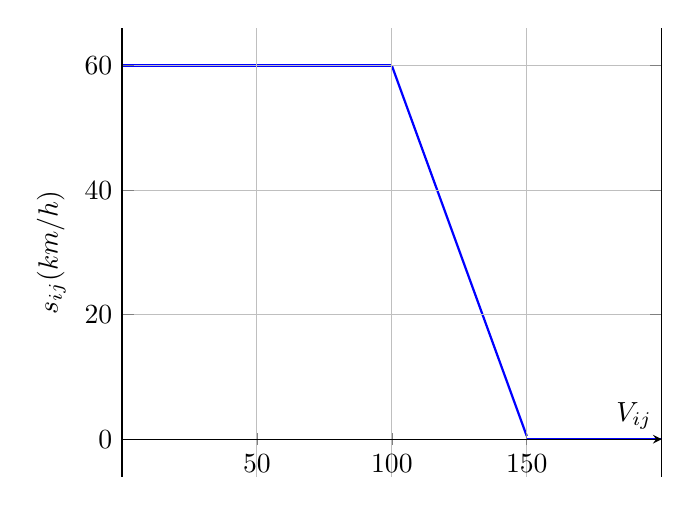
\begin{tikzpicture}
		\begin{axis}[
			xlabel={$V_{ij}$},
			ylabel={$s_{ij} (km/h)$},
			domain=0:250, % adjust the domain based on your preference
			samples=40,
			grid=both,
			axis x line=middle,
			%ymin=-1, % Set the minimum y-axis value
			%ymax=1.4, % Set the maximum y-axis value
			axis on top,
			legend pos=north east
			]
			% Piecewise function
			\addplot[blue, thick, domain=0:100] {60};
			\addplot[blue, thick, domain=100:150] {60 - 1.19*(x-100)};
			\addplot[blue, thick, domain=150:200] {0};
			%\addlegendentry{B}
		\end{axis}
	\end{tikzpicture}
	\caption[Cruising speed in function of traffic density]{Cruising speed in function of traffic density. In this example, $l_{ij} = 60 km/h,V_{ij}^{th} = 100$,$V_{ij}^{max} = 150$ and $\epsilon = 0.5$. }
	\label{fig:speed_model}
\end{figure}
This allows to effectively track the position of the vehicle in terms of time as well. However, the position should be tracked only if the vehicle is currently driving on the street. Therefore, the equation propagating the position of $a$ over $\langle i,j\rangle$ must account for this.
\begin{equation}
	x^a_{ij}(t+\delta) =\begin{cases}
		 x^a_{ij}(t) + s_{ij}(V_{ij}(t))\cdot\delta & \text{if } v^a_{ij}(t) + w^a_{ij}(t)= 1 \\
		 
		 0& \text{if } v^a_{ij}(t) + w^a_{ij}(t)= 0\\
		 0& \text{if }i=j \\
		 %0 & \text{otherwise}
	\end{cases}
	 \label{eq:position_propagation}
\end{equation}
As mentioned above, \equaref{eq:position_propagation} tracks the position of a moving vehicle, i.e., monitors of the state of moving vehicles, and resets it in case a vehicle is not moving anymore.\\
 In addition, the model also needs to track the number of vehicles currently stationed in $i$. This is achieved by introducing an additional variable $f^a_i(t)$, which indicates whether a vehicle arrived at a station $i$. It is defined as following.
\begin{equation}
	f^a_{i}(t) =\begin{cases}
		1 & \text{if }x^a_{ji}(t) \ge d_{ji}\\
		0 & \text{otherwise}
	\end{cases}
	\label{eq:station_propagation}
\end{equation}
This variable can be propagated by introducing two more variables, i.e., $l^a_{ji}$ and $k^a_{ji}$, to indicate whether a vehicle has departed or arrived at a station $i$, respectively. As a result, $f^a_i$ is propagated as follows.
\begin{equation}
		f^a_i(t+1) =f^a_i(t) + \sum_{j\in\mathcal{V}}(k^a_{ji}(t) - l_{ij}^a(t)) 
		\label{eq:stationed_propagation_ind}
\end{equation}
As an additional benefit, \equaref{eq:stationed_propagation_ind} also ensures that a vehicle performs an action on the road $\langle i,j\rangle$ only when stationed at $i$.\\
The variables $l^a_{ji}$ and $k^a_{ji}$ are binary variables as well and their definition is as follows:
\begin{align}
	l^a_{ji}(t) =\begin{cases}
		1 & \text{if }x^a_{ji}(t) \le d_{ji}\\
		0 & \text{otherwise}
	\end{cases}
	\label{eq:departed_variable}
\end{align}

\begin{equation}
	k^a_{ji}(t) =\begin{cases}
		1 & \text{if }x^a_{ji}(t) \ge d_{ji}\\
		0 & \text{otherwise}
	\end{cases}
	\label{eq:arrived_variable}
\end{equation}
The propagation of $k^a_{ji} $ follows a straightforward pattern: if the variable is zero at time $ t $, it can become either one or zero at $ t+1 $, representing the possibility of the vehicle reaching a station or not. However, if $ k^a_{ji}(t) = 1 $ at time $ t $, then $ k^a_{ji}(t+1) = 0 $, indicating a reset. The variable $ l^a_{ji}$ is not propagated, however its definition depends on time. Initially, at $ t=0 $, $l^a_{ji} $ is set to zero, implying no vehicle can start at time zero. At instant $ t+1 $, $l^a_{ji} = 1$ only if the vehicle has moved at time $t$, but was stationed at time $t-1$, otherwise must remain zero\footnote{For a more comprehensive analysis and explanation, please refer to \secref{appendix:sec:propagation_g} and \secref{appendix:sec:definition_p}. }. \\
The definition in \equaref{eq:arrived_variable} imposes that the vehicles must stop if they reached a station. This is translated in \equaref{eq:prop_w} and \equaref{eq:prop_v}
\begin{align}
	w_{ij}^a(t+1) &= \neg v^a_{ij}(t) \land \neg k^a_{ji}(t) \land \neg v^a_{ij}(t) \label{eq:prop_w}\\
	v_{ij}^a(t+1) &= \neg w^a_{ij}(t) \land \neg k^a_{ji}(t) \land \neg w^a_{ij}(t) \label{eq:prop_v}
\end{align}
This formulation leverages the fact that all the above variables are binary. In simple words, this is ensuring that a vehicle can only be rebalancing or driving if it was performing the same action on the previous instance or if it has not arrived at a station yet. In addition, it also ensures that if the vehicle reached a station, then it would stop moving, i.e., $v^a_{ij}(t)=w^a_{ij}(t)=0$\footnote{Please refer to \secref{appendix:sec:const_w_v} for the derivation of these two constraints.}. 

%\begin{equation}
%	f^a_i(t+1) =f^a_i(t) + 1_{d_{ji} \leq x^a_{ji}(t)} - \sum_{j\in\mathcal{V}}(v_{ij}^a + w_{ij}^a) %1_{d_{ji} \neq x^a_{ji}(t)}
%	\label{eq:stationed_propagation_ind}
%\end{equation}

%\begin{equation}
%	f^a_i(t+1) = f^a_i(t) +1_{d_{ji} = x^a_{ji}(t)} - \sum_{j \in \mathcal{N}}( v^a_{ij} + w^a_{ij})
%	\label{eq:stationed_propagation}
%\end{equation}
%The function $1_x$ is commonly known as the indicator function, ing a Boolean variable x that can take values {true, false}. Specifically, $1_x$ is defined as follows:
%\begin{equation}
%	1_x = \begin{cases}
%		1 & \text{if } x \text{ is true} \\
%		0 & \text{if } x \text{ is false}
%	\end{cases}
%\end{equation}
%In other words, $1_x$ equals 1 when x is true and equals 0 when x is false, making it a convenient way to express the truth value of the variable x in mathematical notation.\\
Essentially, for the abovementioned constraint to work, the vehicles can not perform the aforementioned actions, i.e., waiting, routing and rebalancing, at the same time. Furthermore, the vehicles can not perform actions on multiple stations or roads. Therefore, the following constraint is necessary. \\
\begin{equation}
	\sum_{i \in \mathcal{V}}(f^a_{i}(t+1)+\sum_{j \in \mathcal{V}}v^a_{ij}(t) + \sum_{j \in \mathcal{V}}w^a_{ij}(t)) = 1\label{eq:no_3_actions}
\end{equation}
This also implies that, if a vehicle is stationed at a station $i$, it can not have a position anywhere else. 
\begin{equation}
	%0<\sum_{i \in \mathcal{V}}(f^a_{i}(t)+\sum_{j \in \mathcal{V}}\dfrac{x^a_{ij}(t)}{d_{ij}}) \leq1 \label{eq:position_station}
	%d_{ji}
	\sum_{i \in \mathcal{V}}(f^a_{i}(t)+\mathbbm{1}_{ x^a_{ji}(t)\neq 0}) =1 \label{eq:position_station}
\end{equation}
In other words, if a vehicle is travelling through an edge $\langle ji\rangle$, it can only be stationed at $i$ if it finished travelling. \\
 If, on the one hand, it is interesting to know which station is currently hosting which vehicle, it might also be important to know the amount of vehicles currently stationing in the system. This can be achieved by flipping the idea from \equaref{eq:vehicles_on_street} and therefore calculating how many vehicles out of the total number is currently not driving. 
\begin{equation}
	F(t) = |\mathcal{A}| - \sum_{(i,j) \in \mathcal{E}}V_{i,j}(t)%\sum_{i \in\mathcal{N}}\sum_{a \in\mathcal{A}}f^a_{i}
\end{equation}


Denoted by $p_{ij}(t)$ and $g_{ij}(t)$ are the transportation and goods delivery requests respectively starting from station $i$ and headed to $j$. Let $o^p_{ij}(t)$ and $o^g_{ij}(t)$ denoting the number of outstanding requests from $i$ to $j$ for people or goods, respectively, one can describe its propagation as follows:

\begin{equation}
	\begin{aligned}
		o^p_{ij}(t+1) =& o^p_{ij}(t) + p_{ij}(t) - \sum_{a \in \mathcal{A}} P_a\cdot v^a_{ij}(t)\\
			o^g_{ij}(t+1) =& o^g_{ij}(t) + g_{ij}(t) - \sum_{a \in \mathcal{A}} G_a \cdot v^a_{ij}(t)\\
	\end{aligned}
	\label{eq:demand_time}
\end{equation}
%Furthermore, when a vehicle leaves, it can only leave 
It follows then that vehicles can not transport more than what requested, i.e.,:
\begin{equation}
	\begin{aligned}
	 P_a\cdot v^a_{ij}(t) &\leq o^p_{ij}(t) + p_{ij}(t) \forall a \in \mathcal{A} \\
	 G_a \cdot v^a_{ij}(t) &\leq o^g_{ij}(t) + g_{ij}(t) \forall a \in \mathcal{A}
	\end{aligned}
	 \label{eq:no_more_than_request}
\end{equation}
Accordingly, vehicles can rebalance only if there are still requests to be served. 
\begin{equation}
	\begin{aligned}
	 	w^a_{ij}(t) &\leq \sum_{i,j \in \mathcal{E}} (o^p_{ij}(t-1) +o^g_{ij}(t) ) \quad\forall a \in \mathcal{A} \\
		%#G_a \cdot v^a_{ij}(t) &\leq o^g_{ij}(t) + g_{ij}(t) \quad \forall a \in \mathcal{A}
	\end{aligned}
	\label{eq:no_reb_than_request}
\end{equation}

At this point, the definition of the control and the state of the system is complete. More specifically, the state of the system is described by the number outstanding requests, the position of each moving vehicle $x_{ij}(t)$ and the position of each idle vehicle $f^a_{i}(t)$. Let the vector $x$ be the column vector created by reshaping and concatenating $o^p_{ij},o^g_{ij}, x_{ij}^a, f^a_{i}, V_{ij} , k^a_{ij} \text{ and } l^a_{ij}$, the set of feasible states $\mathcal{X}$ is defined as follows. 

\begin{equation}
	\begin{aligned}
	\mathcal{X} &:= \left\{
	\begin{aligned}
		& o^p_{ij} \in (\mathbb{N}_0)^{|\mathcal{N}|}, o^g_{ij} \in (\mathbb{N}_0)^{|\mathcal{N}|}, \\
		 x \quad \Bigg| \quad&k^a_{ij}, l^a_{ij},f^a_{i} \in \{0,1\}^{|\mathcal{A}||\mathcal{N}|} \\%, \text{(\ref{eq:departed_variable})}, \text{(\ref{eq:arrived_variable})}, \text{(\ref{eq:stationed_propagation_ind})} \\
		& x_{ij}^a\in (\mathbb{R}_{\ge 0})^{|\mathcal{A}||\mathcal{N}|}, V_{ij} \in \{ a \in \mathbb{N}_0 : a \leq |\mathcal{A}| \}^{|\mathcal{N}|}\\%T^a_{ij} \in [0, \dfrac{d_{ij}}{\epsilon}]^{|\mathcal{V}|}%T^a_{ij} \in (\mathbb{R}_{\ge 0})^{|\mathcal{V}|} \\
	\end{aligned}
	\right\}\\
	&\\
	&\text{where } x = [o^p_{ij},o^g_{ij}, x_{ij}^a, f^a_{i}, V_{ij} , k^a_{ij}, l^a_{ij}]^T
\end{aligned}
\end{equation}
Note that $o^p_{ii} = 0$ and $o^p_{ii} = 0$. \\
%Note that because of \equaref{eq:prop_w} \equaref{eq:prop_w}, the set of feasible states is time-dependent. 
Similarly, considering the control inputs $v^{a}_{ij}(t)$ and $w^{a}_{ij}(t)$, one can derive the set of feasible control set $\mathcal{U}(t)$ as follows. 
\begin{equation}
	\mathcal{\mathcal{U}}(t) := \left\{
	\begin{aligned}
		&v^a_{ij} \in \{0,1\}^{|\mathcal{A}||\mathcal{N}|}, v^a_{ii} = 0 \\
		u = [v^{a}_{ij}, w^{a}_{ij}]^T \Bigg|&w^a_{ij} \in \{0,1\}^{|\mathcal{A}||\mathcal{N}|},w^a_{ii} = 0 \\ 
		& \text{(\ref{eq:no_3_actions}),\text{(\ref{eq:no_more_than_request})}, \text{(\ref{eq:no_reb_than_request})}
			%\text{(\ref{eq:prop_w})},\text{(\ref{eq:prop_v})},
		} \\
	\end{aligned}
	\right\}
\end{equation}
Since (\ref{eq:prop_w}) and (\ref{eq:prop_v}) depend on time, $\mathcal{U}(t)$ is also time-dependent. \\
Thanks to these formulations, the system can be written as a linear time-dependent system of the form
\begin{equation}
	x(t+1) = Ax + Bu(t)\label{eq:normal_system}
\end{equation}
where $x \in \mathcal{X}$, $u(t) \in \mathcal{U}(t)$ and $A$ and $B$ are the matrix associated to the coefficients of (\ref{eq:position_propagation}), (\ref{eq:stationed_propagation_ind}) and (\ref{eq:demand_time}). \\
\subsection{Objectives}
Clearly, the main objective is to serve all the outstanding requests. 
\begin{equation}
	J_1(x(t)) = \sum_{i,j \in \mathcal{V}}(o^p_{ij}(t) + o^g_{ij}(t))\label{eq:no_request_left}
\end{equation}
However, the performance of the system can be further optimized if other aspects are considered as well. \\
Since the speed of the vehicles is determined by the number of vehicles on the street, limiting it will improve performance. Vehicles serving requests are responsible for the main objective and their number is directly proportional to the number of outstanding requests. On the other hand, rebalancing vehicles, while helpful in reducing the number of requests, they also contribute to congestions. Therefore, by reducing the number of free vehicles moving at time $t$, the speed of the transporting ones is optimized as a result. 
\begin{equation}
	J_2(x(t)) = \sum_{i,j \in \mathcal{V}}w^a_{ij}(t) %T_{ij}^a
\end{equation}
Therefore, the final stage cost will be a combination of the two described above. 
\begin{equation}
	I(x(t)) = J_1(x(t)) + \lambda \cdot J_2(x(t)) 
\end{equation}
where $\lambda$ is the weight used to determine the influence the rebalancing must have in the system.
\subsection{Model Evaluation}
Some comments are in order. Requests are treated considering customers and goods as single entities. More specifically, if a group consisting of three customers reach a station, this is treated as three individual requests, therefore $p_{ij}(t) = 3$. While this simplifies the model description and reflects the requirements for goods delivery, it would create an inconvenient scenario for traveling customers. As a matter of fact, it is not hard to envision situations where a group of travelers would like to travel together. However, it is out of the scope of this work to treat this scenario. Similarly, this model does not take into account scenarios where $o^p_{ij} <\underset{ a \in \mathcal{A}}{min}(P_a)$. This can be tackled by tracking the capacity that vehicles have left at their disposal.\\
The system described in \equaref{eq:normal_system} implicitly assumes the customer arrival to be known a priori. In order words, this is not treated as noise, but rather as a known quantity. 
\begin{equation}
	x(t+1) = Ax(t) + Bu(t) + w(t)\label{eq:disturbed_mpc_formulation}
\end{equation}
where $x(t) \in \mathcal{X}$, $u(t) \in \mathcal{U}(t)$, $w(t) = [p_{ij}(t)\quad g_{ij}(t)\quad0\quad0 \quad0]^T$ and $A$ and $B$ are the matrix associated to the coefficients of (\ref{eq:position_propagation}), (\ref{eq:station_propagation}) and (\ref{eq:demand_time}). \\
\equaref{eq:disturbed_mpc_formulation} treats customer arrival as noise, or disturbance, which makes reasoning on the system considerably harder. Several techniques (\cite{Campo1987RobustMP}, \cite{LANGSON2004125}) have been proposed to deal with this type of MPC systems, i.e. Robust MPC. Alternatively, some works propose solutions to estimate this quantity using Deep Learning techniques (\cite{9202791}, \cite{8569427}).
However, the analysis of those techniques and their performance in this scenario is out of the scope of this work.
Similarly to \secref{sec:vc_model}, the model must take into account that stations do not have unlimited amount of parking spots. As a consequence, the number of vehicles stationed must be limited accordingly and this is achieved as follows. 
\begin{equation}
	\sum_{a \in \mathcal{A}}f^a_i(t) \leq C_i
	\label{eq:parking_limit}
\end{equation}
where $C_i$ indicates the number of parking spots available at $i$. \\
Furthermore, \equaref{eq:model_bpr_approximation2} imposes an implicit capacity limit on the streets. If $\epsilon=0$ and the limit $V^{max}_{ij}$ was exceeded, then the speed would also be zero. In this condition, the time would not be within the defined bounds, i.e., a constraint is violated. \\
Furthermore, one can also calculate the required time $T_{ij}(t)$ based on the speed approximation, as shown in \equaref{eq:required_time}. 
\begin{equation}
	T_{ij}^a(t) = \begin{cases}
			\dfrac{d_{ij} - x^a_{ij}(t)}{s_{ij}(V_{ij}(t))} &\quad \text{if } x_{ij}^a(t) \in (0,d_{ij})\\
			&\\
			0 &\quad\text{otherwise }
		\end{cases}
	\label{eq:required_time} 
\end{equation}
Since this function fails to satisfy the properties of homogeneity and additivity, it is not linear. Consequently, incorporating this function in the model will result in a non-linear model as well. Therefore, it has been decided to exclude it from the model's formulation.

\section{Problem Formulation}\label{sec:prob_formulat_mpc}
The MPC for the ATS problem is formulated as follows. \\
\begin{definition}{\textit{(MPC for ATS) \\}}
	Given $x(t) \in \mathcal{X}$, determine the controls $u(t), \dots, u(t+N)$ according to the following optimization problem.
	\begin{equation}
		\begin{aligned}
			\underset{\substack{u(t), \dots, u(t+N)}}{\text{\textbf{min}}} \quad & J_f(x(N))+\sum_{t=0}^{N-1}I(x(t)) \\
			\text{\textbf{s.t.}} \quad & x(t+1) = Ax(t) + Bu(t) \\
			& x(t) \in \mathcal{X}, \ u(t)\in \mathcal{U} \\
			%& k = t, \dots, t+N\\
			&x(N) \in \mathcal{X}_f\\
		\end{aligned}
		\label{eq:mpc_ats}
	\end{equation}
	where $J_f(x(t+N))$ is the terminal cost function and $\mathcal{X}_f$ is the terminal set. \\
\end{definition}


As the main goal of this section is to prove the stability of (\ref{eq:mpc_ats}), a proper definition of the final cost and terminal set will facilitate this objective. The strategy used to prove stability is the one described in \secref{sec:stable_mpc_systems}. For this purpose, the terminal set is required to be defined around an equilibrium point $x_\mathcal{E}$. A good candidate for the equilibrium point in such systems can be found by observing that the system remains at an equilibrium whenever no more requests arrive and the are no more outstanding requests within the system. In other words, when 
\begin{align*}
	p_{ij}(t) &=0 \\
	g_{ij}(t) &=0\quad\quad \forall i,j\in\mathcal{V}\\
	o^p_{ij}(t) &=0\\
	o^g_{ij}(t) &=0\\
\end{align*}
By \equaref{eq:demand_time}, this implies that, eventually, no more vehicles will transport goods or people anymore. Furthermore, one can also conclude that vehicles will also stop rebalancing themselves. Therefore, $o_{ij}, x_{ij}^a$ and $V_{ij}$ all assume value zero. However, there is no way of knowing exactly where vehicles are going to be stationed. Nevertheless, since vehicles are not driving, they must be stationed somewhere according to the model. In other words, $f^a_{i}$ could assume any value in $\{0,1\}^{|\mathcal{A}||\mathcal{V}|} $ except $ \{0\}^{|\mathcal{A}||\mathcal{V}|}$. Furthermore, at equilibrium, all the vehicles are stationed. That means, the set of possible values for $f^a_{i}$ is further limited accordingly. To define this set, let's consider a function $n : \mathcal{D}_{f^a_{i}} \rightarrow N$, where $\mathcal{D}'_{f^a_{i}} = \{0,1\}^{|\mathcal{A}||\mathcal{V}|} \setminus \{0\}^{|\mathcal{A}||\mathcal{V}|}$, which sums the number of 1s in the set. With this addition, one can fully define the set of values of $f^a_{i}$ at equilibrium. 
\begin{equation}
\mathcal{D}_{f^a_{i}} := 	\left\{
	x \quad | \quad x \in \{0,1\}^{|\mathcal{A}||\mathcal{V}|}, n(x) = |\mathcal{A}|
	\right\}\label{eq:set_of_fs}
\end{equation}
%($\binom{|\mathcal{A}||\mathcal{V}|}{|\mathcal{A}|}$)
While the set is indeed smaller, it is still quite hard to exactly pin-point a specific equilibrium point, as already mentioned above. The difficulty arises because, out of all the elements in (\ref{eq:set_of_fs}), one can not directly identify the one which describes the system fully without knowing how the system progressed in time. However, one can conclude that the equilibrium points are all elements of the set described in \equaref{eq:final_eq}. 
\begin{equation}
	\mathcal{E} := \left\{
	\begin{aligned}
		& o^p_{ij} \in \{0\}^{|\mathcal{N}||\mathcal{A}|} , o^g_{ij} \in \{0\}^{|\mathcal{N}||\mathcal{A}|} \\
		e = [o^p_{ij},o^g_{ij}, x_{ij}^a, f^a_{i}, V_{ij}]^T \Bigg| &k^a_{ij}, l^a_{ij}\in \{0\}, f^a_{i} \in \mathcal{D}_{f^a_{i}}  \\
		& x_{ij}^a\in\{0\}^{|\mathcal{N}||\mathcal{A}|}, V_{ij} \in \{0\}^{|\mathcal{N}|} \\%, T^a_{ij}\in \{0\}^{|\mathcal{V}||\mathcal{A}|} \\
		%& x_{ij}^a\in (\mathbb{R}_{\ge 0})^{|\mathcal{A}||\mathcal{V}|}, T^a_{ij} \in (\mathbb{R}_{\ge 0})^{|\mathcal{V}|} \\
	\end{aligned}
	\right\}\label{eq:final_eq}
\end{equation}\\
While this could be considered as a candidate for the terminal set $\mathcal{X}_f$, it turns out to be too restrictive. This is due to the fact that it would require all vehicles to be stationed and, therefore, not moving. Some of the conditions, however, can be relaxed by considering some implicit assumptions made during the development of the model. Mainly, vehicles are assumed to be perfect and to never break, therefore, one can consider a request to be satisfied the moment it has been picked up. As a result, while the number of requests is still zero, the conditions for $x_{ij}^a$, $f_{i}^a$, $k^a_{ij}$ and $V_{ij}$ can be relaxed. Furthermore, (\ref{eq:stationed_propagation_ind}) is slightly changed so that vehicles do not leave the station as they arrive. This is achieved by simply setting $\sum_{j\in\mathcal{V}}(l^a_{ji}(N-1))=0$.
\begin{equation}
	f^a_i(N) =f^a_i(N-1) + \sum_{j\in\mathcal{V}}(k^a_{ji}(N-1)) 
	\label{eq:stationed_propagation_ind2}
\end{equation}



\begin{equation}
	\begin{aligned}
	\mathcal{X}_f &:= \left\{
	\begin{aligned}
		& o^p_{ij} \in \{0\}^{|\mathcal{N}||\mathcal{A}|} , o^g_{ij} \in \{0\}^{|\mathcal{N}||\mathcal{A}|} \\
		x_f \quad \Bigg| \quad &k^a_{ij},f^a_{i} \in \{0,1\}^{|\mathcal{N}||\mathcal{A}|}, l^a_{ij}\in \{0\}^{|\mathcal{N}||\mathcal{A}|}\\%\text{(\ref{eq:departed_variable})}, \text{(\ref{eq:arrived_variable})}, \text{(\ref{eq:stationed_propagation_ind2})}  \\
		%& x_{ij}^a\in\{0\}^{|\mathcal{V}||\mathcal{A}|} , T^a_{ij}\in \{0\}^{|\mathcal{V}||\mathcal{A}|} \\
		& x_{ij}^a\in (\mathbb{R}_{\ge 0})^{|\mathcal{A}||\mathcal{N}|}, V_{ij} \in \{ a \in \mathbb{N}_0: a \leq |\mathcal{A}| \}^{|\mathcal{N}|}\\% T^a_{ij} \in [0, \dfrac{d_{ij}}{\epsilon}]^{|\mathcal{V}|}%T^a_{ij} \in (\mathbb{R}_{\ge 0})^{|\mathcal{V}|} \\
	\end{aligned}
	\right\}\\
	&\\
	&\text{where } x_f = [o^p_{ij},o^g_{ij}, x_{ij}^a, f^a_{i}, V_{ij} , k^a_{ij}, l^a_{ij}]^T
	\end{aligned}
	\label{eq:final_x_f}
\end{equation}\\
By construction, therefore, $\mathcal{E} \subset \mathcal{X}_f \subset \mathcal{X}$. \\
In addition, thanks to this definition, another particular situation applies. Since $ x_{ij}^a\in (\mathbb{R}_{\ge 0})^{|\mathcal{A}||\mathcal{V}|}$ and $V_{ij} \in \{ a \in \mathbb{N}_0 : a \leq |\mathcal{A}| \}^{|\mathcal{N}|}$, this allows empty vehicles to be circulating in the system. Moreover, since vehicles are not required to be stationed as the minimum requirement for a request to be satisfied is to be picked up, as long as the capacity of the vehicle stationed in $i$ is enough to cover the request, then the number of outstanding requests will remain zero. 
%\begin{equation}
%\begin{aligned}
%	\sum_{a \in \mathcal{A}} P_a\cdot f^a_{i}(t) &\ge p_{ij}(t) \\
%	\sum_{a \in \mathcal{A}} G_a \cdot f^a_{i}(t) &\ge g_{ij}(t) \quad\quad \forall i,j\in\mathcal{V}\\
%	o^p_{ij}(t) &=0, o^g_{ij}(t) =0\\
%\end{aligned}
%\label{eq:conserved_rela}
%\end{equation}
In order to keep the number of outstanding requests to zero, the particular case where the capacity of the vehicles leaving the station us exactly equal to the new demand, i.e.,
%Furthermore, at each time, it is required that the capacity of the vehicle leaving a station is equal to the new demand, as the number of outstanding requests is zero. 
\begin{equation}
	\begin{aligned}
		\sum_{a \in \mathcal{A}} P_a\cdot v^a_{ij}(t) &=  o^p_{ij}(t) \\
		\sum_{a \in \mathcal{A}} G_a \cdot v^a_{ij}(t) &=  o^g_{ij}(t)
	\end{aligned}
	\label{eq:no_more_than_request_f}
\end{equation}
Vehicles, however, can only leave a station if they are present at that station. On the same note, since there must be enough vehicles at every station to serve the requests, those must be rebalanced in such a way that, once a request arrives, a vehicle is ready to serve it. \\
%This function must express then need to ''conserve'' the relation in \equaref{eq:conserved_rela}, which has the by product of also satisfying \equaref{eq:no_more_than_request}.\\
 Furthermore, as a vehicle leaves a station, another vehicle must take its place. Therefore, the follow relation must also hold. 
 \begin{equation}
 	\begin{aligned}
 		P_a\cdot v^a_{ij} &\leq \sum_{j \in\mathcal{V}} \sum_{a'\in \mathcal{A} \setminus \{a\}}P_{a'}\cdot	w^{a'}_{ji}\\
 		G_a\cdot v^a_{ij} &\leq \sum_{j \in\mathcal{V}} \sum_{a'\in \mathcal{A} \setminus \{a\}}G_{a'}\cdot w^{a'}_{ji}\\
 	\end{aligned}
 	\label{eq:replace_vehicle}
 \end{equation}
\equaref{eq:replace_vehicle} is used to ensure that, if a vehicle leaves a station, it must be replaced by one or more vehicles with at least the same capacity.\\

A remark is required. \equaref{eq:no_more_than_request_f} and \equaref{eq:replace_vehicle} indeed allow vehicles to be replaced and, therefore, potentially take care of the requests. However, in addition to the assumption made for \equaref{eq:no_more_than_request_f}, the system will remain in $\mathcal{X}_f$ only as long as the requests are made within a time interval corresponding to the time required to travel from any station containing a free vehicle to the station where the request is starting. In other words, this is a very particular case of extrogenous requests and therefore, for the rest of this section, the external arriving requests will be considered as zero, i.e., $o^p_{ij}(t) = o^g_{ij}(t) = 0$, therefore treating the system as undisturbed. \\
In this case, one can assume that, at the end of a long enough horizon , all the requests are served and no more transporting vehicles $v^a_{ij}$ leaves a station and, likewise, since no more requests are going to arrive, then the number of new rebalancing vehicles $w^a_{ij}$ will also reach zero eventually. 
\subsection{Controller Stability}
As indicated in \secref{sec:stable_mpc_systems}, the three main requirements for controller stability are \textit{(i)} that the control law is feasible considering $\mathcal{U}$, \textit{(ii)} the terminal cost function is Lyapunov and \textit{(iii)} the set $\mathcal{X}_f$ remains feasible.\\
 The control law that must be designed is a function mapping $\mathcal{X}_f$ to a subset of $\mathcal{U}$, i.e., $\kappa_f:\mathcal{X}_f \rightarrow\mathcal{U}_{\kappa_f} \subseteq \mathcal{U}$. Due to \equaref{eq:no_more_than_request} and \equaref{eq:no_reb_than_request}, $\mathcal{U}_{\kappa_f} = \mathcal{U}$, which satisfies the first condition. %, the abovementioned assumptions allow to determine a simpler subset for it, namely \equaref{eq:subset_uk}, which basically reflects that no more vehicle should be moving if all of them arrived.

%\begin{equation}
%	\mathcal{\mathcal{U}}_{\kappa_f}(t) := \left\{
%	\begin{aligned}
%		&v^a_{ij} \in \{0\}^{|\mathcal{A}||\mathcal{V}|} \\
%		u = [v^{a}_{ij}, w^{a}_{ij}]^T \Bigg|&w^a_{ij} \in \{0,1\}^{|\mathcal{A}||\mathcal{V}|}\\ 
%		& \text{(\ref{eq:no_3_actions}),\text{(\ref{eq:no_more_than_request})}, \text{(\ref{eq:no_reb_than_request})}
%			%\text{(\ref{eq:prop_w})},\text{(\ref{eq:prop_v})},
%		} \\
%	\end{aligned}
%	\right\}\label{eq:subset_uk}
%\end{equation}
% It is trivial to demonstrate that $\mathcal{\mathcal{U}}_{\kappa_f}(t) \subseteq \mathcal{U}$.\\ %By construction \equaref{eq:no_3_actions} and \equaref{eq:no_more_than_request} are satisfied. \\
While it is usually difficult to construct a Lyapunov terminal cost function, since the system considered is undisturbed, one can construct a cost function satisfying the Lyapunov properties by observing the vehicles still in motion at the end of the horizon. Since all the requests are taken care of, new vehicles are not put in motion. Hence, all the vehicles still moving, will eventually come to a stop to a station. \\
In this scenario, two candidates can be determined. Firstly, if the traveling time $T_{ij}^a$ has been included in the model, this can be used to determine a cost function $J_t(x)$, which can be proven to be Lyapunov\footnote{The definition and proof can be found in \secref{appendix:sec:lyapunovitity_time} }. Alternatively, an immediate candidate is the number of vehicles still moving in the system. The terminal cost function $J_v(x)$ is trivial to define. \\
\begin{equation}
	 J_v(x(N)):= \sum_{i,j \in \mathcal{V}}V_{ij}\label{eq:cost_function_v}
\end{equation}
With these assumptions proving $J_v(x)$ to be Lyapunov is straight forward. \\

\begin{proposition}{}
	Within the definition of $\mathcal{X}_f$, (\ref{eq:cost_function_v}) is a Lyapunov Function in $\mathcal{X}_f$
\end{proposition}\\
\textit{Proof. } Considering an equilibrium point $x_{\mathcal{E}}\in\mathcal{E}$, three conditions must be met.\\
\begin{enumerate}
	\item The function must be strictly positive except at $x_{\mathcal{E}}$, i.e.,
	\begin{equation*}
		\sum_{i,j \in \mathcal{V}}V_{ij}(t) >0
	\end{equation*}
	This is indeed satisfied by definition of $\mathcal{X}_f$. More specifically, when the system is not at $x_{\mathcal{E}}$, then there are vehicles stll moving, hence $\sum_{i,j \in \mathcal{N}}V_{ij} >0$. 
	\item Secondly, the function must assume the value of zero at equilibrium. ln other words, given the point $x_{\mathcal{E}}$
	\begin{equation*}
		J_v(x_{\mathcal{E}}) = 0
	\end{equation*}
	At equilibrium, there are no vehicles moving. Clearly, the terminal cost function is zero. 
	\item $J_v$ must decrease $\forall x \in \mathcal{X}_f$. 
	\begin{equation*}
		J_v(x(k+1)) - J_v(x(k))\leq 0
	\end{equation*}
	Let's consider a system with only one vehicle $a$ still moving. If the vehicle is not rebalancing or transporting a customer, it can be considered at equilibrium, hence $\sum_{i,j \in \mathcal{N}}V_{ij} =0$ . $J_v$ does not increase nor decrease with time, hence the condition is satisfied. If the vehicle is moving, since it can not move backwards, as time increases, by propagation of $x_{ij}^a$, its position always increases until $x_{ij}^a \ge d_{ij}$. During this time window, $\sum_{i,j \in \mathcal{N}}V_{ij} =1$, eventually reaching the station $j$ and therefore not being in motion anymore, hence the condition remains satisfied. For a system composed of more vehicles, regardless of whether on the same link or not, the same discussion applies. More specifically, since the number of moving vehicles can not increase, can only decrease or remaining the same, hence the condition remains satisfied.
\end{enumerate}


In order to prove stability of (\ref{eq:mpc_ats}), it is imperative to first demonstrate the feasibility of the state sets $\mathcal{X}$ and $\mathcal{X}_f$\footnote{\secref{appendix:feasibility_x_xf_time} contains the same proof for the sets including traveling time as well. The proof in this section works in with those definitions as well} .\\
For the rest of this section, the notation will be eased as follows. 
\begin{align*}
	x &= x(t)\\
	u &= u(t)\\
	x^+ &= x(t+1)
\end{align*} 

\begin{proposition}{(Feasibility of $\mathcal{X}$)}\label{pro:feas_x}
	Let $x \in \mathcal{X}$ and $u \in \mathcal{U}(t)$, then $x_+ \in \mathcal{X}$
\end{proposition}\\
\begin{proof}
 Let $x^+ = [o_{ij}^{p+}, o_{ij}^{g+}, x_{ij}^{a+}, f^{a+}_{i}, V_{ij}^{+}, g^{a+}_{ij}, p^{a+}_{ij}]^T$ and $u = [v^{a}_{ij}, w^{a}_{ij}]^T$. Since $u \in \mathcal{U}$, then \equaref{eq:no_more_than_request} is satisfied, hence $o_{ij}^{p+}, o_{ij}^{g+} \in (\mathbb{N}_0)^{|\mathcal{V}|}$. Trivially, by construction $V_{ij}^{+}$ is also $\in \mathcal{X}$. Likewise, $g^{a+}_{ij}, p^{a+}_{ij} \in \{0,1\}$ because of (\ref{eq:arrived_variable}) and (\ref{eq:departed_variable}). \\
The condition $f^{a+}_{i} \in \{0,1\}^{|\mathcal{A}||\mathcal{V}|}$ can be proven with the help of \equaref{eq:stationed_propagation_ind}. At first vehicles are either present at a station $i$ or not. If vehicles are not stationed, then no action can be taken due to \equaref{eq:no_3_actions} (if $u \in \mathcal{U}$, then it is satisfied), which implies no vehicle is departing or arriving at the station. Otherwise, if vehicles are indeed stationed, then $f^{a}_{i} = 1$. If a vehicle moves, i.e., if $w^a_{ij}(t) = 1$ or $v^a_{ij}(t) = 1$, because of the first condition of \equaref{eq:position_propagation}, then because of \equaref{eq:departed_variable} and (\ref{eq:arrived_variable}) being mutually exclusive, at the next step $f^{a+}_{i} =0$. If, on the other hand, the vehicle is approaching the station, i.e., $f^{a}_{i} =0$ and 
either $v^a_{ji}(t) = 1$ or $w^a_{ji}(t) = 1$, then the following unfolds. If $x_{ij}^{a} \leq d_ij$, $f^{a+}_{i} =0$. Assuming $x_{ij}^{a} \ge d_{ij}$, then $g^{a+}_{ij} = 1$, due to \equaref{eq:stationed_propagation_ind}, then either $f^{a+}_{i} =1$ if $v^a_{ji}(t) = w^a_{ji}(t) = 0$, or $f^{a+}_{i} =0$, if $v^a_{ji}(t) = 1$ or $w^a_{ji}(t) = 1$, which would imply $p^{a+}_{ij}=1$. \\
 $x_{ij}^{a+}\in (\mathbb{R}_{\ge 0})^{|\mathcal{A}||\mathcal{V}|}$ is proved by observing $x_{ij}^a$ in  \equaref{eq:position_propagation}. In case $v^a_{ij}(t) + w^a_{ij}(t)= 0$, the condition is satisfied, since  $x_{ij}^{a+} = 0$.  On the other hand, in case of $v^a_{ij}(t) + w^a_{ij}(t)= 1$, the condition is satisfied according to the definition of $s_{ij}$ and $V_{ij}(t)$.\\
 \end{proof}

\begin{proposition}{(Feasibility of $\mathcal{X}_f$)}\label{pro:feas_xf}
	Let $x \in \mathcal{X}_f$ and $\kappa_f(x) \in \mathcal{U}_{\kappa_f}(t)$, then $x_+\in \mathcal{X}_f$
\end{proposition}\\

\begin{proof}
 Let $x^+ = [o_{ij}^{p+}, o_{ij}^{g+}, x_{ij}^{a+}, f^{a+}_{i}, V_{ij}^{+}, g^{a+}_{ij}, p^{a+}_{ij}]^T$ and $\kappa_f(x) = [v^{a}_{ij}, w^{a}_{ij}]^T$. Since the system is treated as undisturbed, $o_{ij}^{p+}= o_{ij}^{g+},=0$. Because $\kappa_f(x) \in \mathcal{U}_{\kappa_f}(t)$, then \equaref{eq:no_more_than_request_f} is satisfied, implying there is no vehicle leaving the station to serve a request. By construction $V_{ij}^{+}$ is also $\in \mathcal{X}_f$. Likewise, $g^{a+}_{ij}\in \{0,1\}$ because of (\ref{eq:arrived_variable}). \\
If $w^a_{ij} = 0$ , then nothing happens within the system, therefore all the vehicles remain at the station, then $ f^{a+}_{i} \in \{0\}^{|\mathcal{V}||\mathcal{A}|}$ $\forall i \in \mathcal{V}$. Consequently  $x_{ij}^{a+} = 0$, i.e., $\in \mathbb{R}_{\ge 0}$.\\
If vehicles are in movement, i.e., $w^a_{ij} = 1$, a similar argument to the one proposed for the feasibility of $\mathcal{X}$ can be made. Because of \equaref{eq:stationed_propagation_ind}, $f^{a+}_{i}=0$ and $x_{ij}^{a+}\in (\mathbb{R}_{\ge 0})^{|\mathcal{A}||\mathcal{V}|}$, by definition of $s_{ij}$ and $V_{ij}(t)$. Eventually, as the vehicle approaches the station, $d_{ji} = x^a_{ji}(t)$, then $f^{a+}_{i}=1$ due to \equaref{eq:stationed_propagation_ind} and $p^{a+}_{ij}=0$. Since 
\equaref{eq:no_3_actions} is respected ($\kappa_f(x) \in \mathcal{U}_{\kappa_f}(t)$), then (\ref{eq:position_station}) is also respected, as $ w^{a+}_{ij}=0 \implies x_{ij}^{a+}=0$. Condition (\ref{eq:replace_vehicle}) is always respected, assuming there is no new requests. \\
\end{proof}
 Proving that $\mathcal{X}$ and $\mathcal{X}_f$ are feasible provides several insights and assurances regarding the performance of the controller as well. First of all, it implies the controller can always find a feasible solution within these sets, given any initial condition and prediction horizon. This is crucial for ensuring that the controller can operate under various circumstances without violating any constraints. Furthermore, it suggests that the controller can adequately predict future system behavior and plan control actions to ensure that the system remains within safe operating limits. Additionally, it suggests that even in the presence of disturbances or uncertainties, the MPC controller can maintain feasibility by adjusting control actions within the given constraints, which contributes to the robustness of the control system. \\
 More importantly, these can be used to prove the closed-loop stability of the controller. \\

 


\begin{proposition}{(Stability of \ref{eq:mpc_ats})}\\

	Given $\mathcal{X}_f$and $J_f$ defined in (\ref{eq:final_x_f}) and (\ref{eq:cost_function_v}), respectively, and let $\kappa_f:\mathcal{X}\rightarrow\mathcal{U}_{\kappa_f}$, then the controller defined in (\ref{eq:mpc_ats}) is stable in the sense of Lyapunov.
\end{proposition}\\
\begin{proof}
 To prove stability, one must (1) prove the recursive feasibility of $\mathcal{X}_f$ and (2) that the optimal cost function $J*$ is Lyapunov .
\begin{enumerate}
	\item As stated by Proposition \ref{pro:feas_x}, $\mathcal{X}$ is feasible. Let $x\in \mathcal{X}$ and $[u^*_0, u^*_1, \dots, u^*_{N-1}]$ be an optimal control sequence calculated at $x$. At $x^+$ the control sequence $[u^*_0, u^*_1, \dots, \kappa_f(x^*_N)]$ is feasible. This is because $x_N\in \mathcal{X}_f$ and, therefore, $x_+=Ax^*+B\kappa_f(x^*_N) \in \mathcal{X}_f$, since $\mathcal{X}_f$ is feasible, as proven in Proposition \ref{pro:feas_xf}. This proves recursive feasibility.
	\item Given the optimal cost function
	\begin{equation*}
	J^*(k) = J_f(x^*_N)+\sum_{i=0}^{N-1}I(x^*_i, u^*_i)
	\end{equation*}
	At $x(k+1) = x^*_1$, the following needs to be shown
	\begin{equation*}
		J^*(k+1) \leq \widetilde{J}(k)
	\end{equation*}
	where $\widetilde{J}(k)$ is the candidate function and calculated at $\widetilde{U} = \{u^*_1, u^*_2, \dots, \kappa_f(x^*_N)\}$. Therefore
	\begin{align*}
		J^*(k+1) \leq& \sum_{i=1}^{N-1}I(x^*_i, u^*_i) + I(x^*_N, \kappa_f(x^*_N)) + J_f(Ax^*_N + B \kappa_f(x^*_N))\\
		J^*(k+1) \leq& \sum_{i=1}^{N-1}I(x^*_i, u^*_i) +I(x^*_0, u^*_0)-I(x^*_0, u^*_0) + J(x^*_N, \kappa_f(x^*_N)) + J_f(Ax^*_N + B \kappa_f(x^*_N))\\
		J^*(k+1) \leq& \sum_{i=0}^{N-1}I(x^*_i, u^*_i) -I(x^*_0, u^*_0) + I(x^*_N, \kappa_f(x^*_N)) + J_f(Ax^*_N + B \kappa_f(x^*_N))\\
		\text{Since }&J^*(k) = J_f(x^*_N)+\sum_{i=0}^{N-1}I(x^*_i, u^*_i)\\
		J^*(k+1) \leq& J^*(k) -I(x(k), u^*_0)+ \underset{\leq 0 \text{ because $J_f$ is a Lyapunov function}}{\underbrace{J_f(Ax^*_N + B \kappa_f(x^*_N)) + I(x^*_N, \kappa_f(x^*_N)) - J_f(x^*_N)}}\\
		\implies& J^*(k+1) - J^*(k) \leq -I(x(k), u^*_0) \quad I(x,u) >0 \text{ for }x,u \neq 0
	\end{align*}
	As a result, the optimal cost is a Lyapunov function. \\
\end{enumerate}
Hence, one can conclude that the system is asymptotically stable. 
\end{proof}



\newpage


\section{Reduced Connectivity Schema }\label{sec:gts_mpc}
The Reduced Connectivity Schema (RCS) serves to introduce an additional layer of abstraction above the road network, aimed at minimizing the nodes and edges within the graph representation of the network. This abstraction is driven by the understanding that in optimization models, which is the case for the MPC in this work, a decrease in the number of variables facilitates the identification of an optimal control input set. The RCS enables more scalable solutions, particularly in large urban areas or networks with complex topology. It allows optimization algorithms to handle larger networks without sacrificing performance or requiring prohibitively high computational resources. Furthermore, simplifying the network representation through RCS can enhance the robustness of control strategies against uncertainties or disturbances in the system. With fewer variables to optimize, the control system may be more resilient to unexpected events such as sudden changes in traffic conditions or road closures. To achieve these objectives, the RCS must be dynamically constructed depending on how the system evolves. For this purpose, the RCS will be constructed using GTS. Formally, RCS is defined as follows. \\

\begin{definition}{\textit{Reduced Connectivity Schema (RCS)}\\}
	Let $G = (\mathcal{V},\mathcal{E},\mathcal{L}^\mathcal{V},\mathcal{L}^\mathcal{E},s,t)$ be a labelled graph representing a road network of an urban environment. The Reduced Connectivity Schema (RCS) is itself a graph $H = (\mathcal{V}_h,\mathcal{E}_h,\mathcal{L}^\mathcal{V}_h,\mathcal{L}^\mathcal{E}_h,s_h,t_h)$, where $\mathcal{V}_h \subseteq \mathcal{V}$, $\mathcal{E}_h \subseteq \mathcal{E}$, $\mathcal{L}^\mathcal{V}_h \subseteq \mathcal{L}^\mathcal{V}$, $\mathcal{L}^\mathcal{E}_h \subseteq \mathcal{L}^\mathcal{E}$ and $s_h, t_h : \mathcal{E}_h \rightarrow \mathcal{V}_h$ are the source and target functions restricted to edges in $\mathcal{E}_h$, obtained according to a sequence of transformation rules $\mathcal{T}$.
\end{definition}\\

Edges and nodes are labelled according to a simple schema. Let $\mathcal{L}^\mathcal{V}$ be the set of node labels, the latter are labelled as necessary, in case they represent a drop-off or pick-up point, or as simple nodes. On the other hand, $\mathcal{L}^\mathcal{E}$ is the set of edge-labels and include all the distances from each node. \\
The transformation rules in the sequence $\mathcal{T}$ are defined as follows.\\

\begin{roadrule}{ Important Node Reconnection \\}
	If a node is labelled as necessary, then all of its immediate connections are restored. 
	\begin{center}
		\begin{tabular}{|c|c|}
			\hline
			LHS&RHS\\
			\hline
			\begin{minipage}{0.45\textwidth}
				\begin{tikzcd}
					\cdots \arrow[r, ,bend left]&A \arrow[l, bend left] 
				\end{tikzcd}
			\end{minipage}
			&
			\begin{minipage}{0.45\textwidth}
				\begin{tikzcd}
					 & &B \\
					\cdots \arrow[r, ,bend left]&A \arrow[ur, "d_1"]\arrow[rd,"d_3"] \arrow[r,"d_2"]\arrow[l, bend left]&C \\
					&& D
				\end{tikzcd}
			\end{minipage}\\
			\hline
			\multicolumn{2}{|l|}{\textbf{NAC}: A is a dropoff or pick-up node}\\
			\hline
		\end{tabular}
	\end{center}
	\label{rule:imp_reconnection}
\end{roadrule}



\begin{roadrule}{ Simple Node Reconnection \\}
	If a node is labelled as simple, then three of its immediate connections are restored. 
	\begin{center}
		\begin{tabular}{|c|c|}
			\hline
			LHS&RHS\\
			\hline
			\begin{minipage}{0.45\textwidth}
				\begin{tikzcd}
					\cdots \arrow[r, ,bend left]&A \arrow[l, bend left] 
				\end{tikzcd}
			\end{minipage}
			&
			\begin{minipage}{0.45\textwidth}
				\begin{tikzcd}
					& &B \\
					\cdots \arrow[r, ,bend left]&A \arrow[ur, "d_1"]\arrow[rd,"d_3"] \arrow[r,"d_2"]\arrow[l, bend left]&C \\
					&& D
				\end{tikzcd}
			\end{minipage}\\
			\hline
			\multicolumn{2}{|l|}{\textbf{NAC}: A is neither a dropoff nor pick-up node}\\
			\hline
		\end{tabular}
	\end{center}
	\label{rule:simple_connection}
\end{roadrule}

Critically, the difference between \ruleref{rule:imp_reconnection} and \ruleref{rule:simple_connection} lies in the fact that, while \ruleref{rule:imp_reconnection} restores all connections, \ruleref{rule:simple_connection} restores only a fixed amount, which in this case is three. These rules are meant to be applied to expand the connections between necessary with the aim of reducing the unnecessary edges from the original graph. \\
Although this would effectively reduce the number of edges and nodes, other rules can be used to further trim the unnecessary complexity.\\

\begin{roadrule}{Stright Line Simplification\\}
	If three consecutive nodes (A, B, C) form a straight line and B has degree 2, remove node B.
	\begin{center}
		\begin{tabular}{|c|c|}
			\hline
			LHS&RHS\\
			\hline
			\begin{minipage}{0.45\textwidth}
				\begin{tikzcd}
					A \arrow[r, "d_1"] & B \arrow[r,"d_2"] & C \arrow[r, ,bend left] & \cdots \arrow[l, bend left] 
				\end{tikzcd}
			\end{minipage}
			&
			\begin{minipage}{0.45\textwidth}
				\begin{tikzcd}
					A \arrow[r, "d_1 + d_2"] & C \arrow[r, bend left] & \cdots \arrow[l, bend left] 
				\end{tikzcd}
			\end{minipage}\\
			\hline
			\multicolumn{2}{|l|}{\textbf{NAC}: B is not a dropoff nor pick-up node}\\
			\hline
		\end{tabular}
	\end{center}
	\label{rule:straight_line_sim}
\end{roadrule}

\begin{roadrule}{Node Removal based on Neighborhood\\}
	If there exist four nodes ( A, B, C, D ), each connected by exactly one edge, then any node with a degree of two can be removed\footnote{This rule is applied to the four vertices, for clearity the definition of only one case is showed}.
		\begin{center}
			\begin{tabular}{|c|c|}
				\hline
				LHS&RHS\\
				\hline
				\begin{minipage}{0.45\textwidth}
					\begin{tikzcd}
						\cdots\arrow[r, bend left]&\arrow[l, bend left] A \arrow[r] \arrow[d]& B\arrow[d] &\\
						\cdots\arrow[r, bend left]&\arrow[l, bend left]C \arrow[r] & D\arrow[r, bend left] & \cdots \arrow[l, bend left] 
					\end{tikzcd}
				\end{minipage}
				&
				\begin{minipage}{0.45\textwidth}
					\begin{tikzcd}
						\cdots\arrow[r, bend left]&\arrow[l, bend left] A \arrow[d] \arrow[rd]& &\\
						\cdots\arrow[r, bend left]&\arrow[l, bend left]C \arrow[r] & D\arrow[r, bend left] & \cdots \arrow[l, bend left] 
					\end{tikzcd}
				\end{minipage}\\
				\hline
				\multicolumn{2}{|l|}{\textbf{NAC}: B is not a dropoff or pick-up node}\\
				\hline
			\end{tabular}
		\end{center}
		\label{rule:node_removal}
	\end{roadrule}

\begin{roadrule}{Dead-End Removal\\}
	If node B is labelled as simple and has a degree of one, then it can be removed.
	\begin{center}
		\begin{tabular}{|c|c|}
			\hline
			LHS&RHS\\
			\hline
			\begin{minipage}{0.45\textwidth}
				\begin{tikzcd}
					\cdots\arrow[r, bend left]&\arrow[l, bend left] A \arrow[r]& B 
				\end{tikzcd}
			\end{minipage}
			&
			\begin{minipage}{0.45\textwidth}
				\begin{tikzcd}
					\cdots\arrow[r, bend left]&\arrow[l, bend left] A 
				\end{tikzcd}
			\end{minipage}\\
			\hline
			\multicolumn{2}{|l|}{\textbf{NAC}: B is not a dropoff or pick-up node}\\
			\hline
		\end{tabular}
	\end{center}
	\label{rule:dead_end_rem}
\end{roadrule}

As a result of the application of the abovementioned rules, the RCS is constructed and can be used to manage the ATS. \\
Although these rules are highly context-dependent and, as a consequence, other rules could be constructed based on the specific road network, the defined transformation rules offer a versatile framework for tailoring the construction of the RCS to specific urban environments and optimization objectives. By allowing customization based on factors such as traffic patterns, infrastructure layout, and control requirements, the RCS can effectively capture the unique characteristics of different transportation networks. This flexibility ensures that the schema remains adaptable to evolving urban landscapes and diverse application scenarios. \\
An important trade-off between complexity and performance must be considered. By carefully balancing the reduction of unnecessary edges and nodes with the preservation of essential connections, the RCS optimizes network representation to enhance computational performance without compromising control effectiveness. This balance ensures that the resulting schema remains efficient and scalable, capable of supporting real-time decision-making in dynamic urban environments. The balance, however, is difficult to find and, while it is usually determined through iterative refinement and validation, in practice it is difficult to establish a metric or an automatic process for it. 




%\begin{roadrule}{Stright Line Simplification\\}
%	If three consecutive nodes (A, B, C) form a straight line and B has degree 2, remove node B.
%	\begin{center}
%		\begin{tabular}{|c|c|}
%			\hline
%			LHS&RHS\\
%			\hline
%			\begin{minipage}{0.45\textwidth}
%				\begin{tikzcd}
%					A \arrow[r, "d_1"] & B \arrow[r,"d_2"] & C \arrow[r, ,bend left] & \cdots \arrow[l, bend left] 
%				\end{tikzcd}
%			\end{minipage}
%			&
%			\begin{minipage}{0.45\textwidth}
%				\begin{tikzcd}
%					A \arrow[r, "d_1 + d_2"] & C \arrow[r, bend left] & \cdots \arrow[l, bend left] 
%				\end{tikzcd}
%			\end{minipage}\\
%			\hline
%			\multicolumn{2}{|l|}{\textbf{NAC}: B is not a dropoff nor pick-up node}\\
%			\hline
%		\end{tabular}
%	\end{center}
%\end{roadrule}



\section{Use Case Analysis}\label{sec:use_case_mpc}
The use case has been developed using the same data \secref{sec:use_case_analysis_ats} with two main goals in mind. First, the theoretical insights about the stability of the controller need to be confirmed. The hypothesis is that, if the model has full knowledge of the future requests, then an optimal control law should be found such that minimizes the cost function defined in \equaref{eq:no_request_left} and all the vehicles end at a station, i.e., no more moving vehicle is present. Secondly, the model's performance needs to be evaluated using real-world data to determine if it is feasible for application. A summary of the parameters and the performance of the simulations can be found in \tabref{tab:mpc_simulation_comparison}. 



	\begin{table}[h]
		\centering
		\begin{subfigure}{0.5\textwidth}
			\centering
			\begin{tabular}{ |l| c|c|c|}
				\hline
				& 1 & 2&3\\
				\hline
				AVs \#& 30&-&-\\
				Horizon (h) & 3 &-& -\\
				Threshold (km/h) & 60&-&-\\
				Requests & 240&-&-\\
				Road (km) & 30&R&-\\
				
			\end{tabular}
			\caption{ }
			\label{tab:mpc_simu}
		\end{subfigure}%
		\begin{subfigure}{0.5\textwidth}
			\centering
			\begin{tabular}{ |p{2.6cm}|c|c|c|}
				\hline
				& 1 & 2  &3\\
				\hline
				ATT	(\%)		&33&36& 3\\
				ART	(\%)		&17&14 &3\\
				Required AVs			&19&12& 10\\
				Carrying AVs			&13&11&4\\
				Rebalancing AVs			&11&12 &9\\
			\end{tabular}
			\caption{ }
			\label{tab:performance_simulation_mpc}
		\end{subfigure}
		\caption[Various information about the MPC simulations]{Various information about the MPC Simulations. \subfigref{tab:mpc_simu} includes the main details of the various MPC Simulations. ``-'' means the entry has not been changed from the previous one, while ``R'' indicates the real road length is used. All the vehicles can host two travelers and carry 10 pieces of cargo. \subfigref{tab:performance_simulation_mpc} summarizes the performance of the controller during the simulations. The entry ``ATT'' and ``ART'' stand for ``Average Transporting Time'' and ``Average Rebalancing Time'', respectively, and indicate the percentage of time which vehicles spend transporting requests, or rebalancing, on average, while the entry ``Required Vehicles'' represents the number of unique vehicles required during the whole shift, therefore it is not the sum between ``Carrying'' and ``Rebalancing Vehicles''.}
		\label{tab:mpc_simulation_comparison}
	\end{table}
As shown in \tabref{tab:mpc_simu}, all parameters are uniform between the two simulations except for the length of the road, where, for Simulation 1, has been chosen a fixed value for the road length, while for Simulation 2 the real length is used. As a result, the performance of the simulations are slightly different. Although in both cases the same number of requests has been fulfilled, the simulation using the real network demonstrates slightly better results. This discrepancy stems from the fact that, while the average length remains consistent, specific roads exhibit significantly shorter distances. This means, in the same shift duration, vehicles might travel less to fulfill the requests and likewise they need to travel less to rebalance in order to fulfill future requests. Nevertheless, although the vehicles travel less, the number of served requests did not improve. As a matter of fact, the two simulation show that only around ~20\% of the total number of travelers and goods could be transported, which is the result of a short horizon. Due to the random nature of the requests, their destination could be considerably far from where vehicle as stationed. Although a lot of solutions proposed either assume vehicles to be scattered around the area and/or the fleet to be infinitely large, in this work vehicles are stationed only within specified location within the road network, namely the depots. This is more representative of a real world scenario, especially if road parking is wished to be reduced. Furthermore, this situation also highlights problems which would not otherwise be presented. More specifically, most of the requests could not be fulfilled as their pick-up or destination point is too far from where vehicles are stationed in terms of traveling times. It is worth noting that this problem is more present within large urban environment, such as NYC, and it is less visible within small centers. While, intuitively, this could be solved by extending the horizon, this would hinder the performance of the controller, especially for large road network and real-time operations. In other words, extending the horizon is not a scalable solution. This further motives the introduction of the RCS described in \secref{sec:gts_mpc}. This technique offers a mean to further streamline the road network by identifying redundant or inefficient connections, as well as trimming the unnecessary ones, thereby enhancing the overall efficiency and performance of the controller. By trimming the unrequired roads from the network, the number of variables is drastically reduced, which decreases the computational requirements of the optimization problem, allowing to consider a considerably longer horizon. In order to obtain the RCS, the rules included in \secref{sec:gts_mpc} are applied according to the order and frequency described in \tabref{tab:rule_app}. The results and the details of the simulation are once again summarized in \tabref{tab:mpc_simulation_comparison}, specifically as simulation number three.
\begin{table}
	\centering
	\begin{tabular}{ |l| c|}
		\hline
		Rule& Frequency \\
		\hline
		\ruleref{rule:imp_reconnection}& 1 \\
		\ruleref{rule:simple_connection}& 3\\
		\ruleref{rule:straight_line_sim}&-\\
		\ruleref{rule:node_removal}&-\\
		\ruleref{rule:dead_end_rem}&-\\
		%\hline
	\end{tabular}
	\caption[Rule application for the construction of the RCS]{Rule application sequence and frequency for the RCS. ``-'' means that the rule has been applied until no more all the nodes are removed.}
	\label{tab:rule_app}
\end{table}

\begin{figure}[th]
	\centering
	\begin{tikzpicture}
		\begin{axis}[
			xlabel={$i$},
			ylabel={$\# \text{ Edges}$},
			minor tick num=1,
			width=7cm,
			xtick={0,1,2,3,4,5,6,7,8},
			%ytick={131,319,487,623,688,745,772},
			]
			\addplot[viridisbluecolor, mark=*] coordinates {
				(0, 21) (1, 131) (2, 319) (3, 487) (4, 623) (5, 688) (6, 745) (7, 772) (8, 776)
			};
			
		\end{axis}
	\end{tikzpicture}
	\caption[RCS dimensions for different applications of \ruleref{rule:simple_connection}]{RCS dimensions for different applications of \ruleref{rule:simple_connection}. ``$i$'' refers to the amount of iterations applying \ruleref{rule:simple_connection}. All the other rules have been applied with the same parameters.}
	\label{fig:rcs_change}
\end{figure}


 Considering the same requests, the RCS used results in a ~60\% reduction of the total dimension of the original road network, which signifies a notable reduction in complexity for both the model and the optimization problem. As a result, the time performance has noticeably improved, while the overall performance did not decrease. As a matter of fact, not only the same number of requests have been served, but vehicles tend to travel less, since less roads are considered, and, on average, less vehicles tend to be used less frequently as well. \\
The main benefit of the RCS, however, is that its dimension is, contrary to the original representation, related to the how far the requests nodes are from the depots. In other words, thanks greatly to its flexibility, the RCS can be dynamically varied in size depending on this distance. In practice, this translates to the possibility of constructing subgraphs around the depots in order to efficiently satisfy the requests. This leads to expect two main benefits. Firstly, if the requests fall within the graph radius, then they can be satisfied. Secondly, the computational time is expected be greatly reduced, as a result of the reduced number of nodes and edges in the graph. In order to control the dimension of the RCS, a key parameter is the number of iterations for \ruleref{rule:simple_connection}. In the previous discussion, this rule has been applied for seven iterations. The influence of various values for this parameters is showed in \figref{fig:rcs_change}. Originally, the graph had ~1200 edges and, as proven by \figref{fig:rcs_change}, it can be reduced to as little as ~18\% of its original size\footnote{Its evolution is depicted in \figref{app:fig:nyc_evolution}}. However, this number greatly depends on two main factors: \textit{(i)} how close the requests' pick-up and drop-off nodes are to the depots and \textit{(ii)} the actual distance associated with the edge. For this use case, each edge is considered to have a length of 30 km, but, in a real-world application, where this value will be different for each road, various other considerations should be made in this regard. Nevertheless, this reduction in complexity allows to better study the performance of the controller in other settings. \figref{fig:vehicle_usage_km_r} and \figref{fig:requests_km_r} depict the performance of the systems as the dimension of the graph is varied. In order to obtain these results, only requests within a certain radious have been accepted. While it is understood that this is an artificial setting, it allows to obtain insights which would otherwise be difficult to capture. All the simulations use a fleet of 20 vehicles for a horizon of 10 hours.\\
\begin{figure}[t]
	\centering
	\begin{tikzpicture}
		\begin{axis}[
			xlabel={Horizon (m)},
			ylabel={$\text{Outstanding Requests }\#$},
			xmin=0, xmax=20,
			ymin=-2,
			xtick={0,2,4,6,8,10,12,14,16,18,20,22},
			%ytick={0,1,2,3,4,5,6,7,8,9,10,11,12,13,14,15,16,17,18,19,20},
			grid=both,
			minor tick num=1,
			width=10cm,
			height=7cm,
			xticklabels={0, 60, 120, 180, 240, 300, 360, 420, 480, 540, 600, 660},
			%ymajorgrids=true,
			%grid style=dashed,
			%mark=*,
			%mark options={blue},
			%legend style={at={(0.5,-0.15)},anchor=north,legend columns=-1},
			%legend style={at={(0.5,-0.15)},anchor=north,legend columns=-1, font=\footnotesize},
			legend style={
				at={(0.5,-0.18)},
				anchor=north,
				legend columns=2,
				legend image post style={scale=0.8} % Adjust the scale as needed
			},
			%legend entries={Plot 1, Plot 2, Plot 3, Plot 4, Plot 5},
			]
			\addplot[viridisbluecolor, mark=*] coordinates {
				(0, 240) (1, 240) (2, 240) (3, 200) (4, 200) (5, 160) (6, 160) (7, 120) (8, 120) (9, 80) (10, 80) (11, 40) (12, 40) (13, 0) (14, 0) (15, 0) (16, 0) (17, 0) (18, 0) (19, 0) (20, 0)
			};
			\addlegendentry{$i=3, r = 30 \text{ km}$}
			\addplot[viridismagentacolor, mark=+] coordinates {
				(0, 240) (1, 240) (2, 240) (3, 232) (4, 224) (5, 192) (6, 184) (7, 152) (8, 144) (9, 112) (10, 104) (11, 72) (12, 64) (13, 32) (14, 24) (15, 2) (16, 2) (17, 0) (18, 0) (19, 0) (20, 0)
			};
			\addlegendentry{$i=3, r = 60 \text{ km}$}
			\addplot[viridisorangecolor, mark=o] coordinates {
				(0, 240) (1, 240) (2, 240) (3, 232) (4, 224) (5, 192) (6, 184) (7, 152) (8, 144) (9, 112) (10, 104) (11, 72) (12, 64) (13, 32) (14, 24) (15, 2) (16, 2) (17, 0) (18, 0) (19, 0) (20, 0)
			};
			\addlegendentry{$i=3, r = 90 \text{ km}$}
			\addplot[viridiscyancolor, mark=x] coordinates {
				(0, 240) (1, 240) (2, 240) (3, 232) (4, 230) (5, 228) (6, 190) (7, 180) (8, 142) (9, 138) (10, 100) (11, 98) (12, 60) (13, 60) (14, 32) (15, 30) (16, 4) (17, 2) (18, 0) (19, 0) (20, 0)
			};
			\addlegendentry{$i=3, r = 120 \text{ km}$}
			\addplot[viridisgreencolor,mark=square] coordinates {
				(0, 240) (1, 240) (2, 240) (3, 224) (4, 224) (5, 214) (6, 214) (7, 190) (8, 188) (9, 156) (10, 150) (11, 116) (12, 110) (13, 78) (14, 74) (15, 46) (16, 42) (17, 14) (18, 10) (19, 0) (20, 0)
			};
			\addlegendentry{$i=2, r = 150 \text{ km}$}
			
			\addplot[viridisbluecolor,mark=square] coordinates {
				(0, 240) (1, 240) (2, 232) (3, 228) (4, 224) (5, 212) (6, 200) (7, 194) (8, 164) (9, 160) (10, 132) (11, 126) (12, 92) (13, 86) (14, 54) (15, 52) (16, 24) (17, 22) (18, 8) (19, 2) (20, 0)
			};
			\addlegendentry{$i=2, r = 180 \text{ km}$}
			
			\addplot[viridismagentacolor,mark=square] coordinates {
				(0, 240) (1, 240) (2, 240) (3, 226) (4, 226) (5, 214) (6, 206) (7, 192) (8, 184) (9, 166) (10, 164) (11, 144) (12, 142) (13, 118) (14, 114) (15, 88) (16, 84) (17, 58) (18, 54) (19, 26) (20, 26)
			};
			\addlegendentry{$i=2, r = 210 \text{ km}$}
			
			\addplot[viridispurplecolor,mark=square] coordinates {
				(0, 240) (1, 240) (2, 240) (3, 224) (4, 224) (5, 210) (6, 204) (7, 182) (8, 174) (9, 148) (10, 144) (11, 122) (12, 118) (13, 88) (14, 82) (15, 50) (16, 42) (17, 14) (18, 8) (19, 0) (20, 0)
			};
			\addlegendentry{$i=4, r = 210 \text{ km}$}
			
		\end{axis}
		
		
		
		
	\end{tikzpicture}
	\caption[Decrease in Number of Requests Over Time]{Decrease in Number of Requests Over Time.``$i$'' refers to the amount of iterations applying \ruleref{rule:simple_connection} and ``$r$'' is the requests radius in kilometers. The horizon is in minutes. }
	\label{fig:requests_km_r}
\end{figure}
Before delving into the details of those figures, however a particular detail must be noted. Since all the requests are artificially picked to be within the considered radius, it was expected the system to be able to serve most of the requests. This is indeed confirmed by \figref{fig:requests_km_r}. This depicts how the number of outstandingrequests decreases over the horizon time. As expected, as long as the requests are within the RCS radius, the system is able to fulfill all of them. Some cases are faster than other due to the distance from the depot to the request locations. This is indeed the case in real-world situations as well. On the other hand, if a request falls outside the RCS radius, the system is not able to fulfill it. This can also be inferred by \figref{fig:vehicle_usage_km_r}. For example, if requests are over 210 kilometers from the depot, the controller using RCS can not serve them. As a result, not all vehicles will be used, as in the case for $i=2$ and $r=210$ in \figref{fig:vehicle_usage_km_r}. Furthermore, by analyzing \figref{fig:vehicle_usage_km_r}, a particular trend emerges. As the radius increases, more vehicles are required to fulfill the requests and this can be deduced by the fact that, as $r$ increase, so do the situations where all the vehicles are deployed. Note that in case of $i=2$ and $r=210$, all the deployable vehicles are indeed deployed for 80\% of the time. If the radius is small, on the other hand, the full capacity of the fleet is deployed for less, as it is in the case of $i=3$ and $r=30$. Specifically in this case, vehicles are also used although, for the interval before, no vehicle was deployed. 




\begin{figure}[t]
	\centering
	\begin{tikzpicture}
		\begin{axis}[
			xlabel={Horizon (m)},
			ylabel={$\text{Vehicle Usage}$},
			xmin=0, xmax=20,
			ymin=-2, ymax=25,
			xtick={0,2,4,6,8,10,12,14,16,18,20,22},
			xticklabels={0, 60, 120, 180, 240, 300, 360, 420, 480, 540, 600, 660},
			%ytick={0,1,2,3,4,5,6,7,8,9,10,11,12,13,14,15,16,17,18,19,20},
			grid=both,
			minor tick num=1,
			width=10cm,
			height=7cm,
			%ymajorgrids=true,
			%grid style=dashed,
			%mark=*,
			%mark options={blue},
			%legend style={at={(0.5,-0.15)},anchor=north,legend columns=-1},
			%legend style={at={(0.5,-0.15)},anchor=north,legend columns=-1, font=\footnotesize},
			legend style={
				at={(0.5,-0.18)},
				anchor=north,
				legend columns=2,
				legend image post style={scale=0.8} % Adjust the scale as needed
			},
			%legend entries={Plot 1, Plot 2, Plot 3, Plot 4, Plot 5},
			]
			\addplot[viridisbluecolor, mark=*] coordinates {
				(0,0) (1,20) (2,20) (3,20) (4,20) (5,20) (6,20) (7,20) (8,20) (9,20) (10,20) (11,20) (12,20) (13,0) (14,4) (15,3) (16,0) (17,0) (18,3) (19,1) (20,0)(21,0) (22,0)
			};
			\addlegendentry{$i=3, r = 30 \text{ km}$}
			\addplot[viridismagentacolor, mark=+] coordinates {
				(0,0) (1,20) (2,20) (3,20) (4,20) (5,20) (6,20) (7,20) (8,20) (9,20) (10,20) (11,20) (12,20) (13,20) (14,15) (15,13) (16,4) (17,6) (18,3) (19,1) (20,0)(21,0) (22,0)
			};
			\addlegendentry{$i=3, r = 60 \text{ km}$}
			\addplot[viridisorangecolor, mark=o] coordinates {
				(0,0) (1,20) (2,20) (3,20) (4,20) (5,20) (6,20) (7,20) (8,20) (9,20) (10,20) (11,20) (12,20) (13,18) (14,14) (15,5) (16,8) (17,6) (18,8) (19,5) (20,0)(21,0) (22,0)
			};
			\addlegendentry{$i=3, r = 90 \text{ km}$}
			\addplot[viridiscyancolor, mark=x] coordinates {
				(0,0) (1,20) (2,20) (3,20) (4,20) (5,20) (6,20) (7,20) (8,20) (9,20) (10,20) (11,20) (12,20) (13,20) (14,20) (15,20) (16,18) (17,9) (18,7) (19,2) (20,0) (21,0) (22,0)
			};
			\addlegendentry{$i=3, r = 120\text{ km}$}
			\addplot[viridisgreencolor,mark=square] coordinates {
				(0,0) (1,20) (2,20) (3,20) (4,20) (5,20) (6,20) (7,20) (8,20) (9,20) (10,20) (11,20) (12,20) (13,20) (14,20) (15,20) (16,18) (17,9) (18,7) (19,2) (20,0) (21,0) (22,0)
			};
			\addlegendentry{$i=2, r = 150\text{ km}$}
			
			\addplot[viridisbluecolor,mark=square] coordinates {
				(0, 0) (1, 20) (2, 20) (3, 20) (4, 20) (5, 20) (6, 20) (7, 20) (8, 20) (9, 20) (10, 20) (11, 20) (12, 20) (13, 20) (14, 20) (15, 18) (16, 12) (17, 10) (18, 9) (19, 3) (20, 0)
			};
			\addlegendentry{$i=2, r = 180\text{ km}$}
			\addplot[viridismagentacolor,mark=square] coordinates {
				(0, 0) (1, 16) (2, 16) (3, 16) (4, 16) (5, 16) (6, 16) (7, 16) (8, 16) (9, 16) (10, 16) (11, 16) (12, 16) (13, 16) (14, 16) (15, 16) (16, 16) (17, 16) (18, 14) (19, 2) (20, 0)
			};
			\addlegendentry{$i=2, r = 210\text{ km}$}
			\addplot[viridispurplecolor,mark=square] coordinates {
				(0, 0) (1, 20) (2, 20) (3, 20) (4, 20) (5, 20) (6, 20) (7, 20) (8, 20) (9, 20) (10, 20) (11, 20) (12, 20) (13, 20) (14, 20) (15, 20) (16, 19) (17, 14) (18, 8) (19, 2) (20, 0)
			};
			\addlegendentry{$i=4, r = 210\text{ km}$}
		\end{axis}
		
		
		
		
	\end{tikzpicture}
	\caption[Evolution of The Vehicle Usage Over Time]{Evolution of The Vehicle Usage Over Time The vehicle usage is calculated as the sum of the vehicles on the street at time $t$. ``$i$'' refers to the amount of iterations applying \ruleref{rule:simple_connection} and ``$r$'' is the requests radius in kilometers. The horizon is in minutes. }
	\label{fig:vehicle_usage_km_r}
\end{figure}

While obtaining real-world data on goods transportation for direct comparison with the simulation may be challenging, using official NYC taxi data can provide insights into the actual performance of the system. According to the NYC government (\cite{nyc_taxi_history}), considering a ten hour shift, taxis carry less than a passenger per day, more specifically, on average taxis carry 0.354 passengers per taxi-hour\footnote{See \secref{appendix:sec:stats_nyc_taxis} for more details}. Considering this as the baseline, one can derive a comparison with the proposed method in this chapter. Considering the same ten hour shift, following the same calculations, the controller is able to serve 0.83 passengers per taxi-hour, which is a 134\% increase in transporting rate. 

















\section{Conclusion}
Although the controller showed promising results, both theoretically and on a practical use case, some considerations are still in order. Firstly, while the stability of the undisturbed controller is necessary, a real world application will likely deal with a noisy system, which, in this context, translates in various aspects. Intuitively, the first aspect is extrogenous requests which are not considered in advanced, which hypothetically, could still be served, albeit with a longer horizon. Secondly, in a more practical view, the model tracks the speed and the position of the vehicles only based on the presence of other vehicles on the road. In reality, other factors are influencing the vehicles' position. However, regarding the model, the primary limitation arguably comes from the model's exclusive focus on the controllable vehicles, neglecting the presence and behaviors of pedestrians and other road users, such as other vehicles or bikers. Integrating additional layers of complexity to account for the dynamic nature of urban environments, such as incorporating pedestrian behavior, road conditions, and interactions with other vehicles, could enhance the model's predictive capabilities and its utility in practical settings. Furthermore, other elements of viability and of the infrastructure should also be taken into account when dealing with urban environments. For example, vehicles such as ambulances, police cars and firefighters, as well as emergency vehicles in generals, must be treated differently than other vehicles. For instance, correctly modeling and controlling traffic in situations of emergency could potentially help saving lives. Additionally, other less urgent, but more common, situations should also be modeled, such as interactions with railways and other means of transportations. Notably, trains have strict deadlines which one must adhere to. While this could potentially be solved with the addition of time windows constraints, as already done in the previous chapter, other ways should be explored to create a more efficient model. \\
The simplistic nature of the model, however, does not necessarily imply limited applicability. On the contrary, although in simulation, the use case demonstrated a robust and performant controller, with the potential of being applied in a closed-loop scenario, where real vehicles can be efficiently guided towards making the best decisions to improve traffic flow in smart cities. 